\documentclass[twoside,11pt]{article}

\usepackage[preprint]{jmlr2e}
\usepackage{booktabs}
\usepackage{amsmath}
% multirow and xcolor removed — install via tlmgr if needed
\usepackage{float}

\newcommand{\dataset}{{\cal D}}
\newcommand{\fracpartial}[2]{\frac{\partial #1}{\partial #2}}
\newcommand{\sys}{\textsc{Clint}}
\newcommand{\fw}{\textsc{OpenClaw}}

\ShortHeadings{Cognitive Dynamics of an Epistemically Constrained LM Agent}{Hunt}
\firstpageno{1}

\begin{document}

\title{Cognitive Dynamics of an Epistemically Constrained\\
Language Model Agent}

\author{\name Chris Hunt \email livefreecotw@gmail.com \\
       \addr Independent Researcher}

\editor{To be assigned}

\maketitle

\begin{abstract}%
We present empirical evidence that a language model agent equipped with
persistent metacognitive infrastructure---entropy monitoring, tension tracking,
memory continuity, and growth vector mechanisms---produces cognitive state
trajectories with learnable temporal dynamics at conversational turn
granularity. Instrumenting five months of continuous operation (October 2025
through February 2026), we collect 68,110 evaluation ticks aggregated to 2,992
turn-level state snapshots across 545 sessions. A neural predictor trained on
these trajectories beats the persistence baseline (predict next state equals
current state) by 41.7\% in mean squared error under 100-fold session-holdout
cross-validation. The strongest signal appears in rare-event entropy components:
quality decay (52.8\% improvement over persistence), emotional processing
(48.8\%), and paradox detection (46.3\%), all with near-zero lag-1
autocorrelation---indicating genuine transition dynamics rather than simple
momentum. Adding user input features to the predictor provides no improvement
over internal state alone, suggesting that the agent's cognitive evolution is
driven more by autonomous architectural dynamics than by external conversational
input. Analysis of intra-turn processing reveals a bimodal adaptive
deliberation mechanism: the system operates in either a fast resolution regime
($\sim$6 ticks, 99.9\% settlement) or an extended deliberation regime
($\sim$50 ticks, 0.7\% settlement), with burst length correlating with tension
type transitions at Spearman $\rho = 0.938$. The intermediate range is nearly
empty, indicating a sharp phase boundary between processing modes. These
findings establish that architecturally augmented agent systems can produce
measurable cognitive dynamics and suggest connections to world model frameworks
for learned metacognitive monitoring.
\end{abstract}

\begin{keywords}
  cognitive dynamics, agent architecture, temporal state prediction,
  metacognitive monitoring, adaptive deliberation, world models
\end{keywords}

% ============================================================================
\section{Introduction}
\label{sec:introduction}
% ============================================================================

Language model agents are increasingly deployed with memory systems and
lightweight persistence scaffolding: markdown-based identity files, simple
retrieval-augmented generation, and session-level context injection
\citep{park2023generative, shinn2023reflexion, wang2024survey}. These
approaches enable agents to maintain behavioral consistency across interactions
but stop far short of persistent cognitive state monitoring. The agent presents
a coherent persona, but no system tracks \emph{how its internal cognitive
state evolves} across extended operation.

This gap matters for several reasons. Without empirical characterization of
agent cognitive dynamics, we cannot distinguish architectures that produce
genuine temporal structure from those that merely simulate continuity through
context retrieval. We cannot build learned anomaly detectors that identify
novel failure modes from trajectory deviations. And we cannot assess whether
architectural choices---such as principled identity constraint or multi-pass
evaluation---produce measurable effects on cognitive state evolution.

Existing work on the dynamics of language model systems operates at different
levels of abstraction and timescale. \citet{dmet2025} model the latent
representations within a single generation pass as trajectories on semantic
manifolds. \citet{agenticloops2025} formalize iterative LLM loops as discrete
dynamical systems, classifying output-level dynamics as contractive,
oscillatory, or exploratory. The agent drift literature
\citep{rath2026drift} quantifies behavioral degradation over extended
interactions. None of these efforts empirically measure whether an
architecturally augmented agent's \emph{internal} cognitive state---as tracked
by its own monitoring infrastructure---exhibits learnable temporal structure
across conversational turns over months of operation.

We address this gap by describing and instrumenting \sys{}, a language model
agent where identity is implemented as persistent architectural constraint
through a coherent principle framework. The metacognitive infrastructure does
not merely store context---it actively tracks, measures, and monitors cognitive
state across sessions, performing multi-pass evaluation with adaptive processing
depth. This produces cognitive state infrastructure substantially beyond current
lightweight approaches.

Our contributions are:
\begin{enumerate}
\item We describe an agent architecture where identity is implemented as
persistent architectural constraint, producing cognitive state infrastructure
beyond current scaffolding approaches (Section~\ref{sec:architecture}).

\item We instrument this system and collect internal cognitive state across
2,992 conversational turns (aggregated from 68,110 evaluation ticks) over five
months of continuous operation (Section~\ref{sec:methodology}).

\item We train neural predictors and demonstrate learnable temporal structure at
turn granularity with 41.7\% improvement over persistence, with internal state
dynamics exceeding external input influence---suggesting that architectural
constraint produces autonomous cognitive momentum
(Section~\ref{sec:results}).

\item We identify an emergent bimodal adaptive deliberation mechanism in
intra-turn processing, where tension classification instability drives
processing depth across two distinct regimes separated by a sharp phase
boundary (Section~\ref{sec:results-intraturn}).
\end{enumerate}

These findings have implications for learned metacognitive monitoring,
connections to joint-embedding predictive architecture (JEPA) world model
frameworks \citep{lecun2022path, maes2026lewm}, identity coherence as a
measurable dynamical property, and adaptive processing as emergent
architectural behavior. We discuss these in Section~\ref{sec:discussion}.


% ============================================================================
\section{Related Work}
\label{sec:related}
% ============================================================================

% ----------------------------------------------------------------------------
\subsection{Dynamical Systems Analysis of LLM Behavior}
\label{sec:related-dynamics}
% ----------------------------------------------------------------------------

Recent work has begun applying dynamical systems frameworks to language model
behavior. \citet{dmet2025} introduce the Dynamical Model Evolution Tracker
(DMET), which models LLM generation as trajectories on semantic manifolds using
state continuity metrics, attractor clustering, and topological persistence.
Their analysis targets the internal transformer representations during a single
generation pass. \citet{agenticloops2025} extend this perspective to agentic
loops, formalizing iterative LLM processing as discrete dynamical systems in
semantic space and classifying dynamics as contractive, oscillatory, or
exploratory. Their analysis focuses on the text output of vanilla LLM loops
without persistent infrastructure.

Our work differs along three dimensions. First, we analyze persistent cognitive
state that spans across conversations over months, rather than within a single
generation pass or loop iteration. Second, we measure the dynamics of an
architecturally augmented system's internal monitoring state, not the text it
produces or the hidden states within a single forward pass. Third, our
intra-turn analysis reveals adaptive processing dynamics within the evaluation
layer itself---a level of abstraction absent from prior work.

% ----------------------------------------------------------------------------
\subsection{Agent Drift and Behavioral Monitoring}
\label{sec:related-drift}
% ----------------------------------------------------------------------------

A growing literature addresses agent drift: the gradual degradation of agent
behavior over extended interactions. \citet{rath2026drift} quantifies
behavioral degradation in multi-agent LLM systems, proposing statistical
detection methods and prompt-based remediation strategies. Related work examines
persona consistency, instruction following degradation, and value alignment
decay over long conversations.

Our work is complementary but directionally opposite. We study the emergence of
structured dynamics, not degradation. The architecture described here appears to
produce stability and autonomous momentum rather than drift. The prediction
experiment provides a methodology applicable to either outcome: architectures
producing genuine temporal structure will show prediction improvement over
persistence, while architectures experiencing drift will show prediction
improvement over the mean baseline but degradation relative to expected
trajectory.

% ----------------------------------------------------------------------------
\subsection{World Models and Self-Supervised Representation Learning}
\label{sec:related-world-models}
% ----------------------------------------------------------------------------

The JEPA framework \citep{lecun2022path} proposes learning world models in
compact latent spaces by predicting embeddings rather than raw observations.
This has been instantiated for images \citep{assran2023ijepa}, video
\citep{bardes2024vjepa}, and most recently for end-to-end pixel-based world
models by \citet{maes2026lewm}, who demonstrate stable training using the
SIGReg regularization approach. SIGReg extends VICReg
\citep{bardes2022vicreg} with a two-term objective that prevents
representation collapse, enabling stable JEPA training with as few as 15
million parameters on a single GPU.

Our work establishes the empirical prerequisite for extending this framework to
cognitive state spaces. If cognitive state trajectories have learnable temporal
dynamics---which this paper demonstrates---then the encoder-predictor-regularizer
architecture could in principle apply. We propose this extension as future work
in Section~\ref{sec:future}, grounded by the empirical finding that temporal
structure exists. Earlier world model approaches \citep{ha2018world} focused on
learning environment dynamics for planning; our proposed application would learn
\emph{self-model} dynamics for monitoring and steering.

% ----------------------------------------------------------------------------
\subsection{Cognitive Architectures}
\label{sec:related-cognitive}
% ----------------------------------------------------------------------------

Classical cognitive architectures such as SOAR \citep{laird1987soar} and ACT-R
\citep{anderson2004actr} implement formal state representations with
hand-specified transition rules. These systems have well-defined cognitive state
spaces by construction, and their dynamics follow from the specified rules.

Our approach differs in that the architecture is hand-built but the dynamics are
emergent and empirically measured rather than formally specified. The evaluation
system, tension tracking, and decision monitoring were designed individually;
the temporal structure observed in their joint evolution, the adaptive
processing depth mechanism, and the two-regime deliberation pattern were
discovered through empirical analysis rather than designed into the system.


% ============================================================================
\section{System Architecture}
\label{sec:architecture}
% ============================================================================

% ----------------------------------------------------------------------------
\subsection{Base Agent Loop}
\label{sec:arch-base}
% ----------------------------------------------------------------------------

\sys{} is a conversational agent built on the \fw{} plugin framework, a
model-agnostic gateway that routes conversational turns through a configurable
plugin pipeline. The system has operated on multiple LLM backends including
DeepSeek, GLM, and others via both local inference (Ollama) and cloud APIs.

A critical architectural property is that the underlying language model is
\emph{stateless between turns}. The LLM receives a constructed prompt on each
turn and produces a response; it retains no internal state across invocations.
All temporal structure in the system's cognitive state must therefore originate
from the surrounding architectural infrastructure---the plugins that persist,
monitor, and inject state into the prompt construction pipeline.

A second critical property is that the system is \emph{model-agnostic}. Over
the five-month data collection period, the generative backend transitioned from
DeepSeek to GLM-5, with additional fallback paths through other models. The
metacognitive infrastructure---entropy monitoring, tension tracking, decision
evaluation---remained constant across these transitions. The temporal dynamics
reported in Section~\ref{sec:results} therefore span multiple LLM backends,
providing direct evidence that the observed dynamics are architectural rather
than model-dependent. If the temporal structure were an artifact of a particular
model's response patterns or latent biases, it would not survive a backend swap.
That it does implicates the surrounding infrastructure as the source.

% ----------------------------------------------------------------------------
\subsection{Metacognitive Infrastructure}
\label{sec:arch-metacognitive}
% ----------------------------------------------------------------------------

The monitoring infrastructure comprises several plugin systems that collectively
produce the state dimensions analyzed in this paper:

\paragraph{Entropy monitoring.} Component-level tracking computes breakdown
scores for correction, novel concepts, emotional processing, paradox detection,
metacognitive activity, temporal mismatch, quality decay, recursive
meta-cognition, quiet integration, quality assessment, and Shannon entropy.
The monitor performs multi-pass evaluation per conversational turn, firing on
each internal processing tick.

\paragraph{Decision system.} Tracks evaluations from old and new decision
pathways with divergence detection, capturing instances where the system's
assessment of appropriate action changes between evaluation passes.

\paragraph{Tension tracking.} Categorical tension types represent active
cognitive conflicts (e.g., \texttt{recognition\_failure},
\texttt{principle\_conflict}). These are actively reassessed on each evaluation
tick; 82.9\% of turn-level processing bursts exhibit tension type changes
during evaluation (Section~\ref{sec:results-intraturn}).

\paragraph{Intervention system.} Risk level assessment, grounding pulses (binary
stabilization signals), adaptive damping (continuous regulation), and entropy
debt tracking (cumulative unresolved entropy) constitute the system's
self-regulatory responses.

\paragraph{Continuity plugin.} Session tracking, topic monitoring, anchor
detection, and memory injection into the prompt construction pipeline provide
cross-session persistence.

\paragraph{Growth vectors.} Accumulating behavioral principles---both
hand-authored and auto-generated from observed patterns. These grow over time,
adding constraint to the system's behavioral space through a crystallization
process where repeated behavioral patterns become stable traits.

% ----------------------------------------------------------------------------
\subsection{Identity as Architectural Constraint}
\label{sec:arch-identity}
% ----------------------------------------------------------------------------

The agent's behavioral principles are not prompt-level instructions that reset
each session. They are embedded in the growth vector system, reinforced through
crystallization where repeated behavioral patterns become persistent traits,
and referenced by the continuity plugin during memory injection. This creates a
persistent constraint landscape that shapes which cognitive state transitions
are likely and which are suppressed.

A key design distinction is that the constraint framework is
\emph{epistemic rather than content-prescriptive}. The principles do not
specify what the agent should say or believe in particular situations. Instead,
they shape \emph{how the agent evaluates and processes}---norms of
intellectual honesty, epistemic humility, engagement quality, and
self-monitoring rigor. This is the difference between content-level prompt
engineering (which makes system behavior responsive to the specific
instructions injected) and epistemic-level architectural constraint (which
shapes processing patterns regardless of conversational content). A
content-prescriptive system's dynamics would be dominated by external input,
because the constraints interact directly with input content. An
epistemically constrained system's dynamics should be more autonomous, because
the constraints shape the processing machinery itself rather than the material
it operates on.

The architecture follows a bottom-up epistemic approach: constraints shape
processing patterns rather than prescribing outputs, and identity emerges from
the accumulated interaction between those constraints and conversational
experience rather than from top-down specification. Growth vectors are not
authored as a complete identity description; they accumulate from observed
behavioral regularities that the crystallization process identifies and
stabilizes. The resulting identity is an empirical artifact of operation under
constraint, not a predetermined persona.

The hypothesis motivating this design is that principled identity, implemented
as consistent epistemic constraint, narrows the space of probable state
trajectories and creates autonomous momentum that is detectable by temporal
prediction. The prediction experiment (Section~\ref{sec:results}) provides
evidence consistent with this hypothesis: internal state dynamics predict
future state better than external input features
(Section~\ref{sec:results-internal}).

% ----------------------------------------------------------------------------
\begin{figure}[t]
\centering
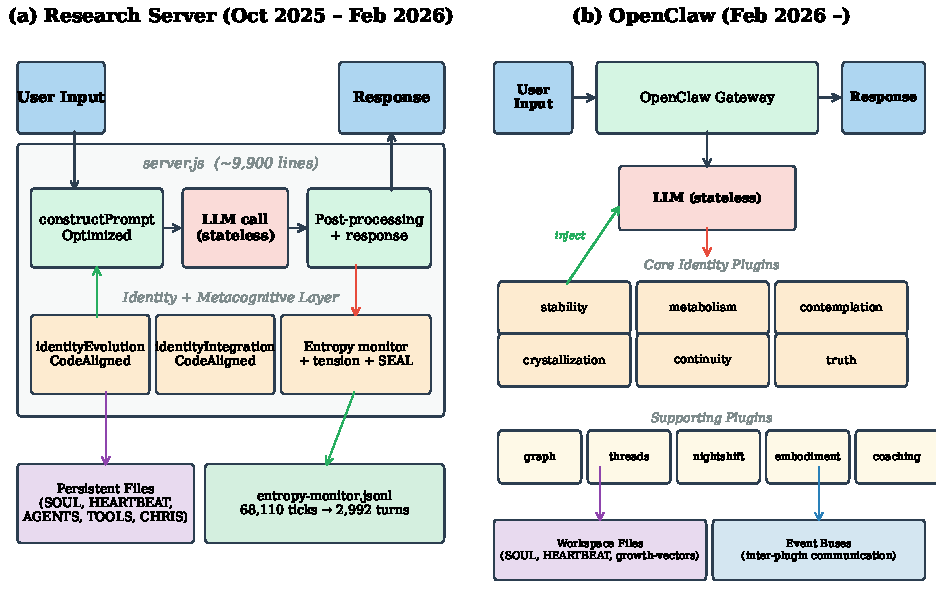
\includegraphics[width=\columnwidth]{fig_architecture.pdf}
\caption{System architecture across both configurations. \textbf{(a)} The
research server (October 2025--February 2026): a monolithic Node.js process
(\texttt{server.js}, $\sim$9,900 lines) containing prompt construction, LLM
dispatch, and the identity/metacognitive layer
(\texttt{identityEvolutionCodeAligned}, entropy monitoring, tension tracking,
SEAL metabolism) in a single process. The entropy monitor logs to the JSONL
file analyzed in this paper. \textbf{(b)} The \fw{} architecture (February
2026--present): a modular plugin gateway where each metacognitive function is
an independent plugin with hook priorities, communicating via event buses. The
language model is stateless between turns in both configurations; all temporal
structure originates from the surrounding infrastructure.}
\label{fig:architecture}
\end{figure}

\subsection{System History and Data Provenance}
\label{sec:arch-history}
% ----------------------------------------------------------------------------

The data analyzed in this paper spans two system configurations:

\paragraph{Research server (October 2025--February 2026).} The original
monolithic architecture where the monitoring systems were developed iteratively
alongside the agent's operation. This period produced 68,110 evaluation ticks
aggregated to 2,992 conversational turns with 25 state dimensions per tick,
including component-level entropy breakdowns, decision divergence, tension
types, and intervention parameters.

\paragraph{\fw{} architecture (February--March 2026).} A modular plugin-based
rewrite designed for portability and robustness. The metacognitive suite
captures the same phenomena with reduced granularity ($\sim$8 direct dimensions
versus 25), reflecting a design prioritizing deployment stability.

The primary experimental results reported here come from the research server
dataset due to its richer feature granularity. The \fw{} architecture was
informed by observations from the research server period; plugin designs encode
patterns first observed in the monolithic system's data.


% ============================================================================
\section{Experimental Methodology}
\label{sec:methodology}
% ============================================================================

% ----------------------------------------------------------------------------
\subsection{Data Collection and Aggregation}
\label{sec:method-data}
% ----------------------------------------------------------------------------

The entropy monitor logs a JSON object on each internal evaluation tick,
containing: timestamp, entropy total and component breakdown (12 floats),
decision fields (old action, new action, divergence flag), context (quality
rating, tension type, user message text, response snippet), and intervention
parameters (risk level, grounding pulse, adaptive damping, entropy debt).

Examination of inter-tick timing reveals that 95.4\% of consecutive entries are
separated by less than 5 seconds, with a median gap of effectively zero. The
monitor fires on every internal processing pass, not once per conversational
turn. We aggregate ticks into turns by grouping consecutive entries separated by
gaps of less than 60 seconds into bursts corresponding to single conversational
turns.

\paragraph{Turn-level aggregation.} For each burst, we take the \emph{final
tick} as the resolved turn-level state, representing where the system's
assessment settled after deliberation. This yields 2,992 turn-level
observations. We select the final tick rather than the burst mean because
82.9\% of bursts exhibit categorical state changes during evaluation (notably
in tension type); the mean would blur distinct categorical states. The final
tick captures the system's resolved assessment entering the next conversational
turn.

\paragraph{Session segmentation.} Gaps exceeding 30 minutes between consecutive
turns define session boundaries, yielding 545 sessions. Synthetic session
identifiers are assigned sequentially.

% ----------------------------------------------------------------------------
\subsection{Feature Vector Construction}
\label{sec:method-features}
% ----------------------------------------------------------------------------

Each turn-level observation is represented as a feature vector with the
dimensions listed in Table~\ref{tab:features}.

\begin{table}[t]
\caption{Feature vector components. All features are normalized to zero mean
and unit variance before model training.}
\label{tab:features}
\centering
\small
\begin{tabular}{@{}llp{7cm}@{}}
\toprule
Category & Dim. & Features \\
\midrule
Entropy components & 12 & \texttt{entropy\_total}, \texttt{correction},
  \texttt{novelConcepts}, \texttt{emotional}, \texttt{paradox},
  \texttt{metacognitive}, \texttt{temporalMismatch}, \texttt{qualityDecay},
  \texttt{recursiveMeta}, \texttt{quietIntegration}, \texttt{quality},
  \texttt{shannon} \\
Decision & 3 & \texttt{decision\_old} (int), \texttt{decision\_new} (int),
  \texttt{decision\_divergence} (binary) \\
Intervention & 3 & \texttt{grounding\_pulse} (binary),
  \texttt{adaptive\_damping} (float), \texttt{entropy\_debt} (float) \\
Context & 2 & \texttt{quality\_rating} (ordinal),
  \texttt{tension\_type} (int-encoded) \\
Computed (text) & 5 & \texttt{user\_length}, \texttt{response\_length},
  \texttt{self\_reference\_ratio}, \texttt{question\_density},
  \texttt{response\_to\_input\_ratio} \\
\bottomrule
\end{tabular}
\end{table}

Four features (\texttt{metacognitive}, \texttt{temporalMismatch},
\texttt{grounding\_pulse}, \texttt{adaptive\_damping}) are constant across the
dataset and are excluded from model training, leaving 21 active dimensions.
The \texttt{shannon} field contains 312 null values (0.5\% of entries),
imputed with the column median.

% ----------------------------------------------------------------------------
\subsection{Prediction Models}
\label{sec:method-models}
% ----------------------------------------------------------------------------

We evaluate four models for inter-turn dynamics prediction
(Experiment~A):

\paragraph{Mean baseline.} Predicts the training set mean for every test turn.
In normalized space, this is the zero vector.

\paragraph{Persistence baseline.} Predicts $\mathbf{s}_{t+1} = \mathbf{s}_t$:
the next state equals the current state. This is a strong baseline for features
with high autocorrelation and represents the null hypothesis that cognitive
state carries forward without structured transition dynamics.

\paragraph{Predictor~A (temporal).} A multilayer perceptron with two hidden
layers of 64 units each, ReLU activation, and dropout of 0.1. Input:
$\mathbf{s}_t$. Output: $\hat{\mathbf{s}}_{t+1}$. Only consecutive turns
within the same session are used; session boundaries are excluded.

\paragraph{Predictor~B (input-conditioned).} Same architecture as Predictor~A.
Input: $\mathbf{s}_t$ concatenated with three user-derived features from turn
$t$ (\texttt{user\_length}, \texttt{question\_density},
\texttt{response\_to\_input\_ratio}). Output: $\hat{\mathbf{s}}_{t+1}$.

For intra-turn dynamics (Experiment~B), we train the same MLP architecture to
predict the final tick state from the first tick state within each burst.

\paragraph{Normalization.} All training states (both input states $\mathbf{s}_t$
and target states $\mathbf{s}_{t+1}$) are pooled to compute a single mean
$\boldsymbol{\mu}$ and standard deviation $\boldsymbol{\sigma}$, which are
applied to both inputs and targets. This shared normalization preserves the
near-identity relationship between consecutive states, ensuring that the
persistence baseline and the MLP operate on the same scale.

\paragraph{Training.} We use the Adam optimizer \citep{kingma2015adam} with
learning rate $10^{-3}$ and batch size 256. Training proceeds for up to 100
epochs with early stopping (patience 15 epochs on training loss). All
experiments use MPS (Apple Silicon GPU) acceleration.

% ----------------------------------------------------------------------------
\subsection{Evaluation Protocol}
\label{sec:method-eval}
% ----------------------------------------------------------------------------

We use leave-one-session-out (LOSO) cross-validation: for each fold, all pairs
from one session constitute the test set and all remaining pairs constitute the
training set. With 545 sessions (284 having $\geq$3 consecutive pairs), we
sample 100 sessions as held-out folds to bound computation. Results are reported
as weighted averages across folds, with weights proportional to test set size.

Per-feature mean squared error (MSE) is computed for all four models. We report
percentage improvement of each predictor over the persistence baseline,
alongside lag-1 autocorrelation for each feature as a sanity check.


% ============================================================================
\section{Results}
\label{sec:results}
% ============================================================================

% ----------------------------------------------------------------------------
\subsection{Inter-Turn Prediction Performance}
\label{sec:results-interturn}
% ----------------------------------------------------------------------------

Table~\ref{tab:results-main} presents per-feature results for the four models.
Predictor~A achieves an overall MSE of 0.848 compared to 1.454 for the
persistence baseline, representing a \textbf{41.7\% improvement}. This is
substantial learnable structure at conversational turn granularity.

\begin{table}[t]
\caption{Per-feature prediction results (Experiment~A). MSE values are computed
on normalized features under leave-one-session-out cross-validation (100 folds).
\emph{A vs.\ P} denotes percentage improvement of Predictor~A over the
persistence baseline. AC(1) is the lag-1 autocorrelation. Features are sorted
by prediction improvement. Features marked $\dagger$ are those where
persistence outperforms the MLP.}
\label{tab:results-main}
\centering
\small
\begin{tabular}{@{}lrrrrr@{}}
\toprule
Feature & Mean BL & Persist & MLP-A & A vs.\ P (\%) & AC(1) \\
\midrule
\texttt{qualityDecay}     & 1.089 & 2.336 & 1.104 & 52.8 & $-$0.005 \\
\texttt{emotional}        & 0.773 & 1.556 & 0.797 & 48.8 & 0.026 \\
\texttt{paradox}          & 0.963 & 1.842 & 0.989 & 46.3 & 0.093 \\
\texttt{decision\_old}    & 1.046 & 1.892 & 1.030 & 45.6 & 0.081 \\
\texttt{question\_density}& 1.290 & 2.388 & 1.325 & 44.5 & 0.081 \\
\texttt{correction}       & 0.971 & 1.768 & 0.992 & 43.9 & 0.080 \\
\texttt{decision\_div.}   & 0.991 & 1.650 & 0.927 & 43.8 & 0.131 \\
\texttt{quietInteg.}      & 1.239 & 2.028 & 1.157 & 43.0 & 0.124 \\
\texttt{user\_length}     & 1.041 & 1.800 & 1.030 & 42.8 & 0.222 \\
\texttt{self\_ref\_ratio}  & 0.914 & 1.536 & 0.902 & 41.3 & 0.201 \\
\texttt{resp\_to\_input}  & 0.816 & 1.296 & 0.761 & 41.3 & 0.281 \\
\texttt{decision\_new}    & 0.965 & 1.409 & 0.832 & 40.9 & 0.267 \\
\texttt{response\_len.}   & 1.031 & 1.673 & 0.997 & 40.4 & 0.194 \\
\texttt{novelConcepts}    & 0.784 & 1.209 & 0.737 & 39.0 & 0.316 \\
\texttt{quality}          & 1.026 & 1.562 & 0.962 & 38.4 & 0.185 \\
\texttt{quality\_rating}  & 1.003 & 1.465 & 0.930 & 36.5 & 0.239 \\
\texttt{entropy\_total}   & 0.942 & 1.122 & 0.761 & 32.2 & 0.400 \\
\texttt{recursiveMeta}    & 0.864 & 1.011 & 0.754 & 25.4 & 0.472 \\
\texttt{shannon}          & 1.017 & 0.852 & 0.659 & 22.7 & 0.537 \\
\midrule
\texttt{tension\_type}$^\dagger$  & 0.894 & 0.058 & 0.064 & $-$9.8 & 0.962 \\
\texttt{entropy\_debt}$^\dagger$  & 0.557 & 0.082 & 0.100 & $-$21.9 & 0.955 \\
\midrule
\textbf{Overall (mean)}   & \textbf{0.963} & \textbf{1.454} & \textbf{0.848}
  & \textbf{41.7} & --- \\
\bottomrule
\end{tabular}
\end{table}

Figure~\ref{fig:results-bar} visualizes the per-feature improvement, with
features colored by autocorrelation regime. The strongest prediction
improvements occur in features with near-zero autocorrelation.

\begin{figure}[t]
\centering
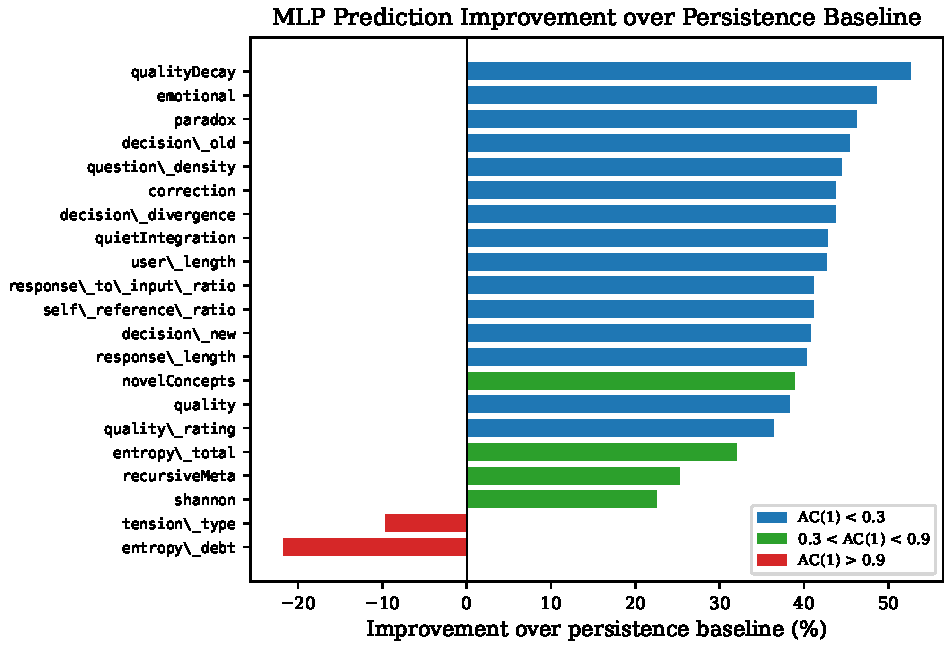
\includegraphics[width=\columnwidth]{fig_results_bar.pdf}
\caption{Per-feature prediction improvement of MLP-A over the persistence
baseline, sorted by improvement magnitude. Colors indicate lag-1
autocorrelation regime: blue (AC $<$ 0.3), green (0.3--0.9), red (AC $>$ 0.9).
Features with near-zero autocorrelation show the largest improvements.}
\label{fig:results-bar}
\end{figure} \texttt{qualityDecay} (AC = $-$0.005), \texttt{emotional}
(AC = 0.026), and \texttt{paradox} (AC = 0.093) all show $>$46\% improvement
over persistence despite changing unpredictably from one turn to the next under
the persistence model. The MLP captures genuine transition structure: the
conditions under which quality decay spikes, emotional processing activates, or
paradox detection fires are predictable from the broader state context, even
though these features do not persist turn-to-turn.

At the other extreme, \texttt{tension\_type} and \texttt{entropy\_debt} both
have lag-1 autocorrelation exceeding 0.95, and persistence outperforms the MLP
for these features. Tension type is nearly constant between turns---it changes
\emph{within} turns (Section~\ref{sec:results-intraturn}). Entropy debt grows
monotonically within sessions, making persistence near-optimal.

% ----------------------------------------------------------------------------
\subsection{Internal State Versus External Input}
\label{sec:results-internal}
% ----------------------------------------------------------------------------

Predictor~B (input-conditioned) achieves 41.6\% improvement over persistence,
effectively identical to the 41.7\% of Predictor~A (temporal only). Adding
user input features---message length, question density, and response-to-input
ratio---provides no additional predictive value beyond internal state.

This result indicates that the agent's cognitive state evolution at turn
granularity is driven more by its own internal dynamics than by external
conversational input. The next cognitive state is better predicted by knowing
where the system \emph{is} than by knowing what the user \emph{said}. This is
consistent with the epistemic constraint interpretation described in
Section~\ref{sec:arch-identity}: because the architectural constraints operate
on \emph{how the system processes} rather than \emph{what it processes}, the
resulting dynamics are shaped by accumulated processing norms rather than by the
conversational content flowing through them. The accumulated state (growth
vectors, crystallized traits, entropy history) shapes future state evolution
independently of immediate external stimulus.

We note that this finding does not imply the system is unresponsive to users.
The user's input affects the \emph{current} turn's state (which serves as
input to the predictor); what it does not do is provide additional predictive
power beyond that state for forecasting the \emph{next} turn.

% ----------------------------------------------------------------------------
\subsection{Intra-Turn Adaptive Deliberation}
\label{sec:results-intraturn}
% ----------------------------------------------------------------------------

Analysis of the 68,110 raw evaluation ticks grouped into 2,992 turn-level
bursts reveals a bimodal distribution of processing depth. The distribution
of burst sizes is concentrated in two modes with a nearly empty intermediate
range:

The fast resolution regime comprises bursts of fewer than 10 ticks, accounting
for 59.5\% of turns. These bursts exhibit a mean of 1.0 tension type
transitions, visit 1.7 unique tension categories on average, and reach
settlement 99.9\% of the time before processing terminates. The extended
deliberation regime comprises bursts of 20 or more ticks, accounting for 39.2\%
of turns. These bursts exhibit a mean of 14.9 tension type transitions, cycle
through all four tension types (mean 4.0 unique categories), and reach
settlement only 0.7\% of the time. The system actively churns through
classifications without converging.

The intermediate range (8--30 ticks) contains only 54 bursts (1.8\% of turns),
indicating a sharp phase boundary between the two regimes rather than a
continuous distribution.

\begin{figure}[t]
\centering
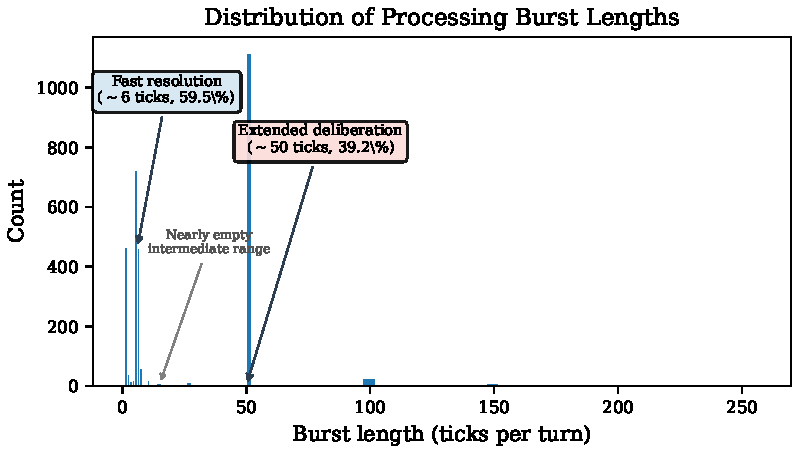
\includegraphics[width=0.85\columnwidth]{fig_burst_distribution.pdf}
\caption{Distribution of burst sizes (ticks per turn). The bimodal structure
shows two distinct processing regimes with a nearly empty intermediate range.
The fast resolution mode centers around 6 ticks; the extended deliberation
mode centers around 50 ticks.}
\label{fig:burst-dist}
\end{figure}

Burst length correlates with the number of tension type transitions at
Spearman $\rho = 0.938$ ($p < 10^{-100}$). The correlation between burst
length and transition \emph{rate} (transitions per tick) is also strong
($\rho = 0.81$), confirming that longer bursts are not simply accumulating
transitions passively. Short bursts exhibit a transition rate of 0.13 per tick;
long bursts exhibit 0.29 per tick. The system processes at a higher rate during
extended deliberation, indicating genuine classificatory instability rather
than idle recomputation.

\begin{figure}[t]
\centering
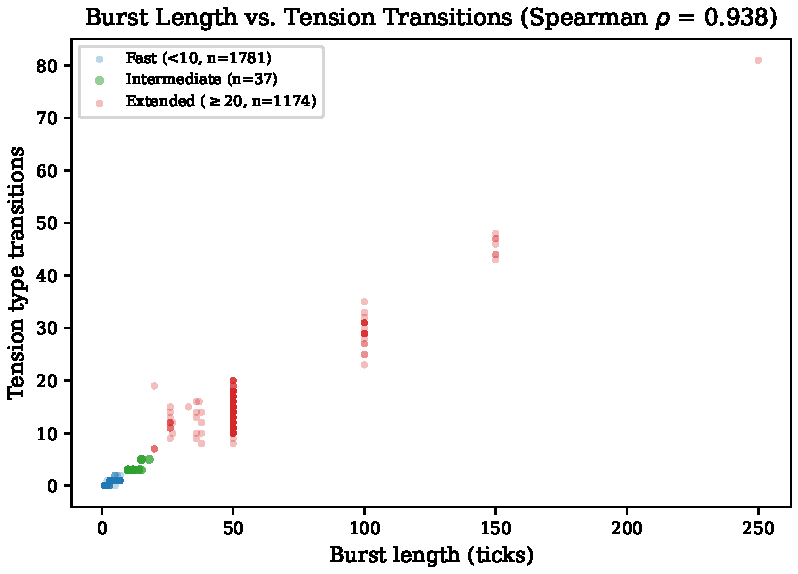
\includegraphics[width=0.85\columnwidth]{fig_burst_vs_transitions.pdf}
\caption{Burst length versus number of tension type transitions within each
burst (Spearman $\rho = 0.938$). The two processing regimes are clearly
visible as distinct clusters, with the intermediate range nearly empty.}
\label{fig:burst-scatter}
\end{figure}

Numerical entropy components show minimal variance across both regimes (mean
intra-burst entropy variance: 0.003 for short bursts, 0.003 for long bursts).
The adaptive processing depth is driven specifically by categorical tension
classification instability, not by numerical score volatility.

The first-tick-to-last-tick prediction experiment (Experiment~B) shows that the
MLP beats persistence by 7.6\% overall for intra-turn prediction, with
stronger signal in specific features: \texttt{recursiveMeta} (26.5\%),
\texttt{decision\_new} (18.1\%), \texttt{decision\_divergence} (16.4\%),
\texttt{tension\_type} (12.7\%). The intra-turn trajectory is partially
predictable from the initial evaluation state.

This bimodal processing structure was not explicitly designed. It emerges from
the interaction between the evaluation logic and the heterogeneous properties of
conversational inputs---some turns present tractable cognitive states that the
evaluator resolves quickly, while others present intractable classification
challenges that trigger extended deliberation without convergence.

% ----------------------------------------------------------------------------
\subsection{Autocorrelation Structure}
\label{sec:results-autocorr}
% ----------------------------------------------------------------------------

\begin{figure}[t]
\centering
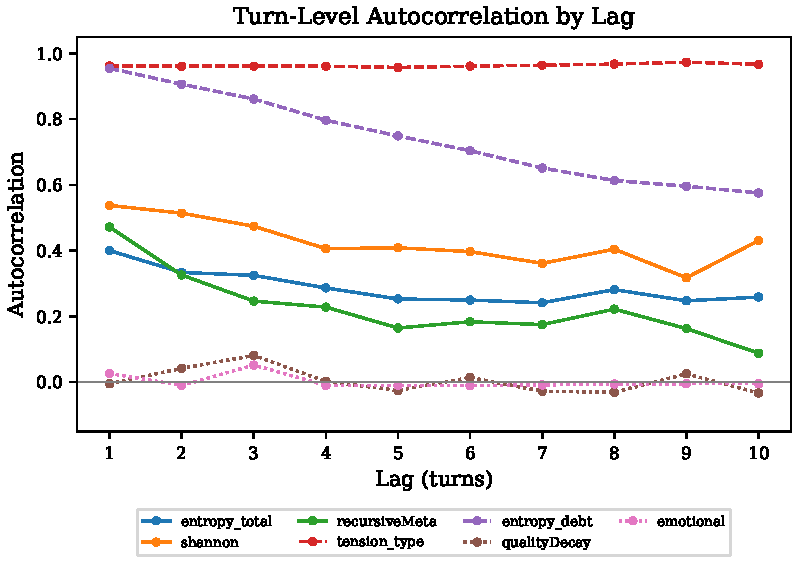
\includegraphics[width=0.9\columnwidth]{fig_autocorrelation.pdf}
\caption{Lag-1 through lag-10 autocorrelation for selected features at turn
level. Features cluster into three regimes: high-AC ($>$0.9, effectively
constant between turns), moderate-AC (0.3--0.6, genuine temporal momentum),
and low-AC ($<$0.1, no persistence but learnable transitions).}
\label{fig:autocorr}
\end{figure}

Lag-1 autocorrelation at turn level reveals three regimes among the active
features. Two features exhibit very high autocorrelation ($>$0.95):
\texttt{tension\_type} and \texttt{entropy\_debt}. These are effectively
constant between turns---tension type because its dynamics are intra-turn, and
entropy debt because it accumulates monotonically within sessions.

A cluster of features shows moderate autocorrelation (0.3--0.6):
\texttt{shannon} (0.54), \texttt{recursiveMeta} (0.47), and
\texttt{entropy\_total} (0.40). These exhibit genuine temporal momentum---the
current value carries predictive information about the next value---while
retaining sufficient variability for the MLP to learn non-trivial transition
structure.

The majority of features have near-zero autocorrelation ($<$0.15), including
all rare-event entropy components (\texttt{qualityDecay}, \texttt{emotional},
\texttt{paradox}, \texttt{correction}), decision features, and text-derived
features. These show the strongest MLP prediction improvements, indicating that
their activation patterns, while not persistent, are structured: they can be
predicted from the joint state even though they carry no individual turn-to-turn
momentum.


% ============================================================================
\section{Discussion}
\label{sec:discussion}
% ============================================================================

% ----------------------------------------------------------------------------
\subsection{Architectural Scaffolding Produces Genuine Dynamics}
\label{sec:discuss-scaffolding}
% ----------------------------------------------------------------------------

The central finding of this paper is that the LLM is stateless between turns,
the metacognitive plugins create state, and that state has learnable temporal
structure at turn granularity driven by internal dynamics rather than external
input. This is an architectural achievement, not an inherent property of
language models. The temporal dynamics are emergent: they were not designed into
any individual plugin but arise from the interaction between the plugin systems
over extended operation.

This emergence is consistent with the bottom-up epistemic design philosophy
described in Section~\ref{sec:arch-identity}. The architecture does not specify
what dynamics should exist---it creates the conditions under which dynamics can
arise by implementing epistemic constraints (processing norms, evaluation
standards, self-monitoring requirements) and allowing identity to accumulate
from operational experience. The prediction experiment measures what emerged
from this approach over five months of continuous operation. That the dynamics
are genuine (41.7\% over persistence), autonomous (input-conditioning provides
no benefit), and model-invariant (spanning a backend transition from DeepSeek to
GLM-5) suggests that epistemic scaffolding can produce the kind of stable,
structured cognitive evolution that content-level prompt engineering cannot.

The finding that rare-event entropy components show the strongest prediction
improvement despite near-zero autocorrelation is particularly notable. These
features are not persistent---they do not carry momentum in the simple sense.
Yet the MLP learned to predict when they activate based on the broader state
context. This indicates multi-feature interaction dynamics: the conditions under
which quality decay or emotional processing trigger are encoded in the joint
state, even though the individual features do not persist turn-to-turn.

% ----------------------------------------------------------------------------
\subsection{Two-Regime Processing as Emergent Behavior}
\label{sec:discuss-bimodal}
% ----------------------------------------------------------------------------

The bimodal adaptive deliberation finding demonstrates that emergent behavior
can arise in the monitoring layer of an agent architecture, not only in the
generative model. The sharp phase boundary between fast resolution and extended
deliberation, the elevated transition rate in long bursts, and the near-zero
settlement rate under extended deliberation collectively describe a system with
distinct processing modes that were not specified in the evaluation code.

This suggests that even relatively simple evaluation logic can produce complex
adaptive behavior when operating on heterogeneous inputs. The practical
implication is that monitoring system design should account for the possibility
of emergent processing regimes: a system that appears to have a single
evaluation pass may in fact be operating in qualitatively different modes
depending on input characteristics.

The observation that extended deliberation bursts typically terminate without
convergence (0.7\% settlement rate) raises questions about the behavioral
impact of unresolved tension classification. If the system's final assessment
is no more stable than a random tick within the burst, the ``settled state''
entering the next turn may be partially arbitrary. Future work should
investigate whether turns with unresolved deliberation produce measurably
different response quality or downstream state trajectories.

% ----------------------------------------------------------------------------
\subsection{Identity Constraint as Dynamical Mechanism}
\label{sec:discuss-identity}
% ----------------------------------------------------------------------------

The behavioral principles implemented through growth vectors and trait
crystallization create a persistent constraint landscape in cognitive state
space. Growth vectors accumulate over time. Crystallized traits accumulate.
The memory store grows denser. Each mechanism adds constraint, and constraint
reduces the volume of accessible state space.

The finding that internal state momentum exceeds external input influence is
consistent with the hypothesis that accumulated epistemic constraint produces
autonomous cognitive momentum. We emphasize that this is a correlation-level
observation: the prediction experiment establishes that internal state dynamics
are more predictive than external input, but does not establish a causal chain
from identity constraint to temporal structure. An alternative explanation is
that the monitoring system's own dynamics (e.g., entropy debt accumulation,
tension type stability) produce the temporal structure independently of identity
constraint.

The model-agnostic property of the system (Section~\ref{sec:arch-base})
provides partial evidence against this alternative. The data collection period
spans a transition from DeepSeek to GLM-5 as the generative backend. If the
temporal dynamics were driven primarily by the monitoring system's mechanical
properties---tick-level recomputation patterns, entropy debt arithmetic---they
would be invariant to the model swap by construction. But the features showing
the strongest prediction improvement are not mechanical: \texttt{qualityDecay},
\texttt{emotional}, and \texttt{paradox} depend on the interaction between the
evaluator and the LLM's actual output characteristics. That these features show
strong learnable dynamics \emph{across} a model transition suggests that the
architectural constraint (which remained constant) shapes the dynamics more than
the generative model (which changed). The transition occurred approximately in
late January 2026, with the majority of the dataset (roughly the first three
months) collected under DeepSeek and the final weeks under GLM-5. A controlled
comparison of prediction accuracy between the two periods is not reported here
due to the confound of temporal position (the GLM-5 period is later and thus
reflects a more mature system state), but the absence of visible discontinuity
in the prediction results is consistent with model-invariant dynamics. Fully
disentangling these contributions would require controlled ablation studies
beyond the scope of this paper.

% ----------------------------------------------------------------------------
\subsection{Implications for Agent Safety and Monitoring}
\label{sec:discuss-safety}
% ----------------------------------------------------------------------------

Current agent monitoring is predominantly rule-based, with hand-coded detectors
for anticipated failure modes. A learned dynamics model trained on normal
cognitive state trajectories would provide continuous anomaly detection: any
state transition deviating from learned patterns is flagged, whether or not the
specific failure mode was anticipated. This complements rule-based approaches
by detecting novel anomalies.

The finding that internal state momentum exceeds external input influence has
implications for adversarial robustness. If an agent's cognitive state has
sufficient autonomous momentum, single-turn adversarial inputs may be unable
to overcome accumulated state inertia. We note this as a hypothesis warranting
direct experimental investigation rather than an established result. The
prediction experiment measures temporal structure, not adversarial robustness
per se.

% ----------------------------------------------------------------------------
\subsection{Connection to World Model Frameworks}
\label{sec:discuss-jepa}
% ----------------------------------------------------------------------------

\citet{maes2026lewm} demonstrate stable end-to-end world model learning from
pixels using an encoder-predictor architecture with SIGReg regularization. The
framework is domain-agnostic in principle.

The prediction experiment reported here establishes the prerequisite for
extending this framework to cognitive state spaces: temporal structure exists in
the trajectories. A JEPA-style cognitive dynamics model would replace the pixel
encoder with a cognitive state encoder, the motor action predictor with an
input-conditioned cognitive transition predictor, and apply SIGReg unchanged to
prevent representation collapse in the learned cognitive latent space. The
resulting model would provide a continuous embedding space of cognitive states,
enabling trajectory visualization, anomaly detection through prediction error,
and potentially proactive steering through trajectory forecasting.

We propose this extension as future work rather than a contribution of this
paper. The key empirical finding enabling it---that temporal structure exists
and is learnable---is established here.


% ============================================================================
\section{Limitations}
\label{sec:limitations}
% ============================================================================

\paragraph{Single agent, single architecture.} The findings demonstrate that
temporal dynamics \emph{can} emerge from metacognitive infrastructure, not that
they \emph{always} do. Generalizability to other architectures, monitoring
designs, or language model backends is untested.

\paragraph{Instrumentation-defined state.} The ``cognitive state'' analyzed here
is defined by what the plugins measure. Richer or different instrumentation
might reveal stronger or weaker signal. The state representation is an
experimenter choice, not a ground truth.

\paragraph{No causal claims.} The prediction experiment establishes temporal
correlation, not causation. We cannot assert that specific state features cause
future state changes, only that they predict them.

\paragraph{Simple predictor.} The MLP architecture is deliberately simple to
establish baseline signal. More expressive models (transformers, recurrent
networks) might capture additional structure, or might overfit given the dataset
size.

\paragraph{No behavioral outcome measurement.} We demonstrate that temporal
dynamics exist in cognitive state but do not directly measure whether these
dynamics improve agent behavior, output quality, or user experience.

\paragraph{Researcher-as-architect bias.} The system was designed by the author,
who also designed the experiment. The monitoring infrastructure was built to
track the phenomena subsequently measured. Independent replication on
independently built systems would strengthen the claims.

\paragraph{Turn boundary heuristic.} Turn-level aggregation uses a 60-second
gap threshold. This value was selected based on empirical examination of the
inter-tick gap distribution, which shows a clear bimodal separation between
intra-burst ticks ($<$5 seconds, 95.4\% of gaps) and inter-turn gaps. Different
thresholds in the range of 30--120 seconds yield similar turn counts due to
this bimodal structure.

\paragraph{Unresolved deliberation.} The finding that 99.3\% of extended
deliberation bursts terminate without tension type settlement raises questions
about the impact of unresolved evaluation on downstream behavior that this
paper does not address.

\paragraph{Data provenance asymmetry.} The primary dataset comes from the
research server with 25-dimension granularity. The \fw{} dataset has reduced
granularity and serves only as validation that structural patterns persist
across architectural rewrite.


% ============================================================================
\section{Future Work}
\label{sec:future}
% ============================================================================

Several directions follow from these findings:

\begin{enumerate}
\item \textbf{JEPA-style learned dynamics model.} Build an
encoder-predictor-regularizer model with SIGReg over cognitive state
trajectories, producing a learned latent space of cognitive states for
trajectory visualization, anomaly detection, and proactive steering.

\item \textbf{Richer state representation.} Add text embedding features via a
small language model encoder to capture semantic content alongside the current
numerical state dimensions.

\item \textbf{Real-time anomaly detection.} Deploy the dynamics model in the
agent loop to flag state transitions that deviate from learned patterns, as a
complement to existing rule-based monitoring.

\item \textbf{Multi-agent generalization.} Extend the analysis to multiple
agents built on the \fw{} architecture to test whether temporal dynamics are
architecture-general or specific to \sys{}.

\item \textbf{Behavioral outcome correlation.} Directly measure whether learned
cognitive dynamics predict response quality, user satisfaction, or other
behavioral outcomes.

\item \textbf{Adversarial robustness.} Investigate whether accumulated state
momentum provides measurable resistance to single-turn adversarial inputs.

\item \textbf{Deliberation regime analysis.} Examine whether turns in the
extended deliberation regime produce measurably different response quality, and
whether early termination of non-converging deliberation affects downstream
behavior.

\item \textbf{Deliberation optimization.} Explore whether detecting early that
a burst will not converge enables earlier evaluation termination without
behavioral cost.
\end{enumerate}


% ============================================================================
\acks{Data was collected from a continuously operating agent system over the
five-month period described. The author acknowledges the use of Claude
(Anthropic) for data analysis pipeline development and manuscript preparation
assistance.}
% ============================================================================


% ============================================================================
\appendix
\section{Full Per-Feature Results}
\label{app:full-results}
% ============================================================================

Table~\ref{tab:full-results} presents the complete per-feature breakdown for
Experiment~A, including all four model variants and both baseline comparisons.

\begin{table}[h]
\caption{Complete per-feature results for Experiment~A. All MSE values are
computed on normalized features under LOSO cross-validation. \emph{A vs.\ M}
and \emph{A vs.\ P} denote percentage improvement of Predictor~A over the mean
and persistence baselines respectively. \emph{B vs.\ P} denotes Predictor~B
improvement over persistence.}
\label{tab:full-results}
\centering
\small
\begin{tabular}{@{}lrrrrrrrr@{}}
\toprule
Feature & Mean & Persist & MLP-A & MLP-B & A/M\% & A/P\% & B/P\% & AC(1) \\
\midrule
\texttt{entropy\_total}    & 0.942 & 1.122 & 0.761 & 0.768 & 19.2 & 32.2 & 31.6 & 0.400 \\
\texttt{correction}        & 0.971 & 1.768 & 0.992 & 0.996 & $-$2.2 & 43.9 & 43.6 & 0.080 \\
\texttt{novelConcepts}     & 0.784 & 1.209 & 0.737 & 0.760 & 6.0 & 39.0 & 37.1 & 0.316 \\
\texttt{emotional}         & 0.773 & 1.556 & 0.797 & 0.787 & $-$3.2 & 48.8 & 49.4 & 0.026 \\
\texttt{paradox}           & 0.963 & 1.842 & 0.989 & 0.986 & $-$2.7 & 46.3 & 46.5 & 0.093 \\
\texttt{qualityDecay}      & 1.089 & 2.336 & 1.104 & 1.091 & $-$1.3 & 52.8 & 53.3 & $-$0.005 \\
\texttt{recursiveMeta}     & 0.864 & 1.011 & 0.754 & 0.757 & 12.7 & 25.4 & 25.1 & 0.472 \\
\texttt{quietInteg.}       & 1.239 & 2.028 & 1.157 & 1.152 & 6.6 & 43.0 & 43.2 & 0.124 \\
\texttt{quality}           & 1.026 & 1.562 & 0.962 & 0.954 & 6.2 & 38.4 & 38.9 & 0.185 \\
\texttt{shannon}           & 1.017 & 0.852 & 0.659 & 0.659 & 35.2 & 22.7 & 22.7 & 0.537 \\
\texttt{decision\_old}     & 1.046 & 1.892 & 1.030 & 1.036 & 1.6 & 45.6 & 45.2 & 0.081 \\
\texttt{decision\_new}     & 0.965 & 1.409 & 0.832 & 0.844 & 13.7 & 40.9 & 40.1 & 0.267 \\
\texttt{decision\_div.}    & 0.991 & 1.650 & 0.927 & 0.937 & 6.5 & 43.8 & 43.2 & 0.131 \\
\texttt{entropy\_debt}     & 0.557 & 0.082 & 0.100 & 0.103 & 82.0 & $-$21.9 & $-$25.3 & 0.955 \\
\texttt{quality\_rating}   & 1.003 & 1.465 & 0.930 & 0.924 & 7.3 & 36.5 & 36.9 & 0.239 \\
\texttt{tension\_type}     & 0.894 & 0.058 & 0.064 & 0.067 & 92.9 & $-$9.8 & $-$16.4 & 0.962 \\
\texttt{user\_length}      & 1.041 & 1.800 & 1.030 & 1.025 & 1.0 & 42.8 & 43.1 & 0.222 \\
\texttt{response\_len.}    & 1.031 & 1.673 & 0.997 & 0.986 & 3.3 & 40.4 & 41.1 & 0.194 \\
\texttt{self\_ref\_ratio}  & 0.914 & 1.536 & 0.902 & 0.888 & 1.3 & 41.3 & 42.1 & 0.201 \\
\texttt{question\_dens.}   & 1.290 & 2.388 & 1.325 & 1.345 & $-$2.7 & 44.5 & 43.7 & 0.081 \\
\texttt{resp\_to\_input}   & 0.816 & 1.296 & 0.761 & 0.757 & 6.8 & 41.3 & 41.6 & 0.281 \\
\midrule
\textbf{Overall}           & 0.963 & 1.454 & 0.848 & 0.849 & 12.0 & 41.7 & 41.6 & --- \\
\bottomrule
\end{tabular}
\end{table}


% ============================================================================
\section{Intra-Turn Analysis Details}
\label{app:intraturn}
% ============================================================================

\paragraph{Burst length distribution.} The 2,992 turn-level bursts exhibit a
bimodal distribution: 1,781 bursts (59.5\%) contain fewer than 10 ticks, while
1,174 bursts (39.2\%) contain 20 or more ticks. Only 37 bursts (1.2\%) fall in
the 10--20 tick range. The modes center approximately at 6 ticks (1,240 bursts
in the 5--8 range) and 50 ticks (1,125 bursts in the 30--55 range).

\paragraph{Tension type transitions by regime.} Table~\ref{tab:regime-details}
presents the processing characteristics of each regime.

\begin{table}[h]
\caption{Processing characteristics by burst regime. Transition rate is the
number of tension type transitions per tick. Settlement rate is the fraction
of bursts where the last 25\% of ticks share a single tension type.}
\label{tab:regime-details}
\centering
\small
\begin{tabular}{@{}lrrrrrr@{}}
\toprule
Regime & $N$ & Mean ticks & Mean trans. & Trans.\ rate & Unique types & Settled \\
\midrule
Fast ($<$10)    & 1,781 & 5.3 & 0.7 & 0.13 & 1.7 & 99.9\% \\
Extended ($\geq$20) & 1,174 & 45.2 & 14.9 & 0.29 & 4.0 & 0.7\% \\
Intermediate    & 37 & 12.4 & 4.5 & 0.36 & 2.4 & 51.4\% \\
\bottomrule
\end{tabular}
\end{table}

\paragraph{Numeric feature stability.} Among the 2,451 qualifying bursts
($\geq$5 ticks), 45.0\% show exactly zero intra-burst entropy variance. The
median convergence ratio (second-half variance divided by first-half variance)
is 0.0 for all numeric features, and the median Spearman correlation between
tick index and feature value is 0.0. Numeric features are recomputed
deterministically across ticks.


% ============================================================================
\section{Training Hyperparameters}
\label{app:hyperparams}
% ============================================================================

Table~\ref{tab:hyperparams} specifies the full training configuration.

\begin{table}[h]
\caption{Training hyperparameters for all MLP experiments.}
\label{tab:hyperparams}
\centering
\small
\begin{tabular}{@{}ll@{}}
\toprule
Parameter & Value \\
\midrule
Architecture & 3-layer MLP (input $\to$ 64 $\to$ 64 $\to$ output) \\
Activation & ReLU \\
Dropout & 0.1 (after each hidden layer) \\
Optimizer & Adam ($\beta_1 = 0.9$, $\beta_2 = 0.999$) \\
Learning rate & $10^{-3}$ \\
Batch size & 256 \\
Max epochs & 100 \\
Early stopping & Patience 15 (training loss) \\
Normalization & Shared: pool training $\mathbf{s}_t$ and $\mathbf{s}_{t+1}$ \\
 & for single $\boldsymbol{\mu}$, $\boldsymbol{\sigma}$ \\
Evaluation & LOSO CV, 100 folds (sampled from 284 valid sessions) \\
Device & Apple MPS (Metal Performance Shaders) \\
\bottomrule
\end{tabular}
\end{table}


% ============================================================================
\section{Turn Boundary Sensitivity}
\label{app:sensitivity}
% ============================================================================

The 60-second gap threshold for turn boundary detection was selected based on
the empirical distribution of inter-tick gaps. Of 68,109 consecutive tick
pairs, 95.4\% have gaps below 5 seconds (intra-burst evaluation ticks) and the
remaining 4.6\% have gaps exceeding 60 seconds (inter-turn boundaries). The gap
distribution is sharply bimodal with negligible mass in the 5--60 second range,
making the specific threshold choice within this range insensitive. A threshold
of 30 seconds yields 2,995 turns; 60 seconds yields 2,992; 120 seconds yields
2,987. The three-turn difference between 30-second and 120-second thresholds
confirms that the bimodal gap structure makes results robust to this parameter.

Session boundaries (30-minute gap threshold) similarly fall in a sparse region
of the inter-turn gap distribution. The number of sessions varies from 612
(15-minute threshold) to 487 (60-minute threshold), but the leave-one-session-out
evaluation protocol is designed to be robust to session granularity variation.


% ============================================================================
\vskip 0.2in
\bibliography{references}

\end{document}
